\documentclass[oneside, 11pt]{article}

\usepackage[T1]{fontenc}
\usepackage[utf8]{inputenc}
\usepackage[english]{babel}
\usepackage{enumerate}
\usepackage{isotope}


\usepackage{fouriernc}
\usepackage[detect-all, binary-units, separate-uncertainty=true,
            per-mode=symbol, retain-explicit-plus, retain-unity-mantissa=false]{siunitx}

\usepackage{setspace}
\setstretch{1.2}

\setlength{\parskip}{\smallskipamount}
\setlength{\parindent}{0pt}

\usepackage[headheight=14pt]{geometry}
\geometry{marginparwidth=0.5cm, verbose, a4paper, tmargin=3cm, bmargin=3cm,
          lmargin=2cm, rmargin=2cm}

\usepackage{float}

\usepackage[fleqn]{amsmath}
\numberwithin{equation}{section}
\numberwithin{figure}{section}

\usepackage{graphicx}
\graphicspath{{images/}{../../../images/}}

\usepackage{tikz}
\usetikzlibrary{shapes}
\usetikzlibrary{plotmarks}

\newcounter{Exercise}
\setcounter{Exercise}{1}
\usepackage{xcolor}
\definecolor{shadecolor}{gray}{0.9}
\usepackage{framed}
\usepackage{caption}

\usepackage{url}


\usepackage{fancyhdr}
\pagestyle{fancy}
\fancyhf{}
\rhead{\thepage}
\renewcommand{\footrulewidth}{0pt}
\renewcommand{\headrulewidth}{0pt}

\fancypagestyle{firststyle}
{
    \fancyhf{}
    \rhead{\thepage}
    \cfoot{\includegraphics[height=30pt]{HiSPARClogo}}
    \rfoot{\includegraphics[height=25pt]{CCbysa}}
    \lfoot{
\includegraphics[height=30pt]{NIKHEFlogo}}
    \renewcommand{\footskip}{50pt}
    \renewcommand{\footrulewidth}{0.1pt}
    \renewcommand{\headrulewidth}{0pt}
}

\newcommand{\figref}[1]{Figuur~\ref{#1}}

\newcommand{\hisparc}{\textsmaller{HiSPARC}\xspace}
\newcommand{\kascade}{\textsmaller{KASCADE}\xspace}
\newcommand{\sapphire}{\textsmaller{SAPPHiRE}\xspace}
\newcommand{\jsparc}{\textsmaller{jSparc}\xspace}
\newcommand{\hdf}{\textsmaller{HDF5}\xspace}
\newcommand{\aires}{\textsmaller{AIRES}\xspace}
\newcommand{\csv}{\textsmaller{CSV}\xspace}
\newcommand{\python}{\textsmaller{PYTHON}\xspace}
\newcommand{\corsika}{\textsmaller{CORSIKA}\xspace}
\newcommand{\labview}{\textsmaller{LabVIEW}\xspace}
\newcommand{\daq}{\textsmaller{DAQ}\xspace}
\newcommand{\adc}{\textsmaller{ADC}\xspace}
\newcommand{\hi}{\textsc{h i}\xspace}
\newcommand{\hii}{\textsc{h ii}\xspace}
\newcommand{\mip}{\textsmaller{MIP}\xspace}
\newcommand{\hisparcii}{\textsmaller{HiSPARC II}\xspace}
\newcommand{\hisparciii}{\textsmaller{HiSPARC III}\xspace}

\DeclareSIUnit{\electronvolt}{\ensuremath{\mathrm{e\!\!\:V}}}

\DeclareSIUnit{\unitsigma}{\ensuremath{\sigma}}
\DeclareSIUnit{\mip}{\textsmaller{MIP}}
\DeclareSIUnit{\adc}{\textsmaller{ADC}}

\DeclareSIUnit{\gauss}{G}
\DeclareSIUnit{\parsec}{pc}
\DeclareSIUnit{\year}{yr}




%document details
\author{N.G. Schultheiss \\ translated and adapted by K. Schadenberg}
\date{}
\title{Data Processing - Periodic Data}


\begin{document}
\maketitle

\section{Introduction}
Obtaining data from a single HiSPARC detector is very easy. All data is available from \url{http://data.hisparc.nl/} . This module explains how to import the data into a spreadsheet application and perform a number of analyses.

\section{Getting the data}
Data can be downloaded via \url{http://data.hisparc.nl/} . This page shows all registered HiSPARC detectors, active detectors are shown as links. Clicking on a detector link shows the last day with available data. In figure \ref{fig:data_screen} the data from detector 13001, placed at the University of Bristol, from the 1st of November 2012 is shown as an example.

\begin{figure}\begin{center}
\includegraphics[scale=0.6]{Data_HiSPARC_Station_13001.pdf}
\caption{Information available via \protect\url{http://data.hisparc.nl/} .}\label{fig:data_screen}
\end{center}\end{figure}

This page shows the measurement data on the left and the detector settings on the right. Lets start at the top right of the page. The first thing we see is a small calendar. With this calendar we can browse to specific dates and look at the results from that day. The link `Station List' brings us back to the overview of detector stations.

Below the calendar is the position of the detector with a the location on a map.

Below the location some hardware parameters are listed. Station 13001 has four detector plates and thus uses two electronics boxes, one master and one slave. Here you can see the hardware number, its firmware version, and the voltage supplied to the different photomultiplier tubes.

On the left hand side of the page the actual data is shown. There are three graphs:
\begin{description}
\item[Event Histogram] shows the number of registered coincidences per hour.
\item[Pulse height histogram] shows the height of the registered coincidences.
\item[Pulse integral histogram] shows the integral of the registered coincidences.
\end{description}

The data that is used to generate these graphs can be directly downloaded from this site. In the top right corner of every graph there is a link to the source data `Source'. The data is saved in a comma separated value file (.csv). The contents of the file should look something like figure \ref{fig:data_CSV}.\footnote{Windows systems do not always correctly recognise the file settings of the .csv file. If this is the case you should use the second import method for Excel described in this module.} The top of the file gives a short description of the file contents. In the example of figure \ref{fig:data_CSV} the data of 17th of June 2012 by station 13001 is used. It registered 792 coincidences between 2 a.m. and 3 a.m.

\begin{figure}\begin{center}
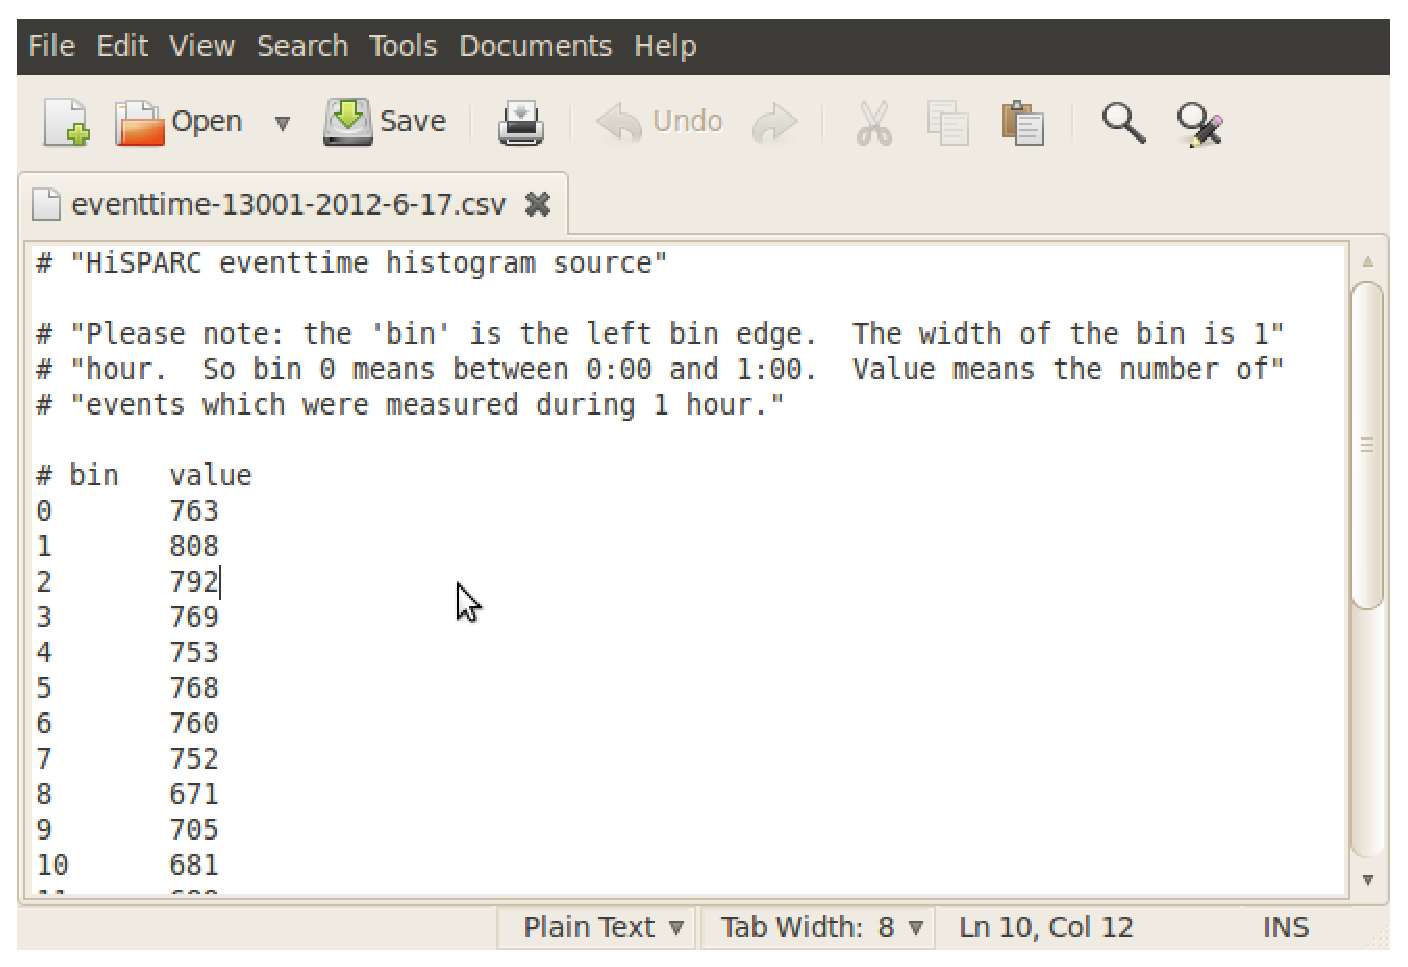
\includegraphics[scale=0.5]{Screenshot_CSV_data_HiSPARC_Station_13001}
\caption{Part of the .csv file.}\label{fig:data_CSV}
\end{center}\end{figure} 

\section{Importing the data}
The process of importing data is described for two different spreadsheet applications: Microsoft Excel and LibreOffice Calc\footnote{There are a few differences between LibreOffice and OpenOffice are, but this manual should be applicable to both.}.

\subsection{Microsoft Excel}
If the .csv file is correctly recognised by Windows then the .csv file can be directly opened by Excel and the the bin number and measurement value will have been placed in separate columns. If this is not the case then the .csv data needs to be manually imported into Excel. To do this follow these steps:
\begin{enumerate}[1.]
\item Start Excel.
\item Select `Data' in the Ribbon (top menu bar).
\item Click on `From text' and select the file you want to import.
\item Excel will now start a Wizard to import the file.
\item Most probably Excel will recognise the correct settings. In step one of the wizard choose `Delimited' as file type. In step two make sure that only the option `Tab' is selected. In step three the `Column data format' should be `General'.
\item After clicking `Finish' you can specify where you want to place the imported data.
\end{enumerate}

\subsection{LibreOffice Calc}
When trying to open the .csv file with Calc the Text Import Wizard should automatically start. Make sure to select `Tab' under `Seperated by' and deselect `Space' (this should be the default setting). Under `Other options' the first option `Quoted field as text' should be selected. Click `OK' an you are done.

\section{Simple data processing}
Now that we have our data we can look patterns and relationships. We could for instance examine if there are more coincidences during the day time, or if the moon influences our measurements. Let's start simple with the determination of the average number of coincidences during one week.

\begin{shaded}
\textbf{Exercise \theExercise \stepcounter{Exercise}} : Download the coincidence data of an entire week, make sure the detector was up and running correctly the entire week.\end{shaded}
\begin{shaded}
\textbf{Exercise \theExercise \stepcounter{Exercise}} : Import the data from the first day and try to recreate the graph from the HiSPARC data site. Remember: a graph always has a title and clear descriptions on the axes.\end{shaded}
\begin{shaded}
\textbf{Exercise \theExercise \stepcounter{Exercise}} : Import the data from the other six days. Copy all the data into a new sheet and place the different days in separate columns. Now calculate the average of every hour. Make a graph of the averages. Are there differences between this graph and the previous graph you made? Can you see a pattern?\end{shaded}
\begin{shaded}
\textbf{Exercise \theExercise \stepcounter{Exercise}} : How would you compare data from two different detector stations? What information about the different detectors is available that could help you explain any differences?\end{shaded}
\begin{shaded}
\textbf{Exercise \theExercise \stepcounter{Exercise}} : If you want to look at possible effects of the moon, what is the minimum amount of time you would have to take data from?\end{shaded}

\section{More advanced data processing}
In the previous section we did some easy data analysis, lets take it a step further. Let's see if we can locate possible sources of cosmic radiation.

In theory the HiSPARC detectors could detect particles coming from any direction. However, because of the geometry of the detectors they are most sensitive to particles coming strait from above. Luckily this is also where most of the showers come from (see module `Airshowers'). Lets assume that all particles we measure at 12 o'clock come from directly above our detector, that would be the direction of the Sun. An hour later our detector has turned away from the Sun and is now looking at a slightly different part of the Sky. 

The Earth rotates both around its own axis and around the Sun. That means that, although at 12 o'clock we will always look at the Sun, the stars will have a slightly different position each day. To take this into account in our calculations we need to use a different time system; celestial or sidereal time (see the module `The Sky' for a bit of background information). 

Every day the Earth completes one revolution around its axis of rotation and every year it makes one revolution around the Sun. If we take the stars as reference point however it seems as though the Earth makes one extra revolution around its axis every year. That is why the \textit{rotation period} as used by astronomers differs from the solar day, it includes that part of the rotation that is needed to accommodate the portion of the \textit{orbital period} during one day.

\begin{shaded}
\textbf{Exercise \theExercise \stepcounter{Exercise}} : Calculate the duration of a sidereal day in solar hours.\end{shaded}

Using this new time system we can try to figure out where cosmic radiation comes from. To do this we will divide the sky into four quadrants and calculate the amount of radiation coming from each of the quadrants using vector decomposition, see figure \ref{fig:measuring_angle}.

Time represents a certain angle with respect to the stars. We can switch between time and angle using the following equation:
\begin{equation} \alpha = 2 \pi \frac{t}{T} \label{eq:time} \end{equation}
$t$ is the time we want to convert into an angle and $T$ is the duration of an entire revolution. Try to figure out for yourself what time we need to use in this equation, solar or sidereal.

\begin{figure}\begin{center}
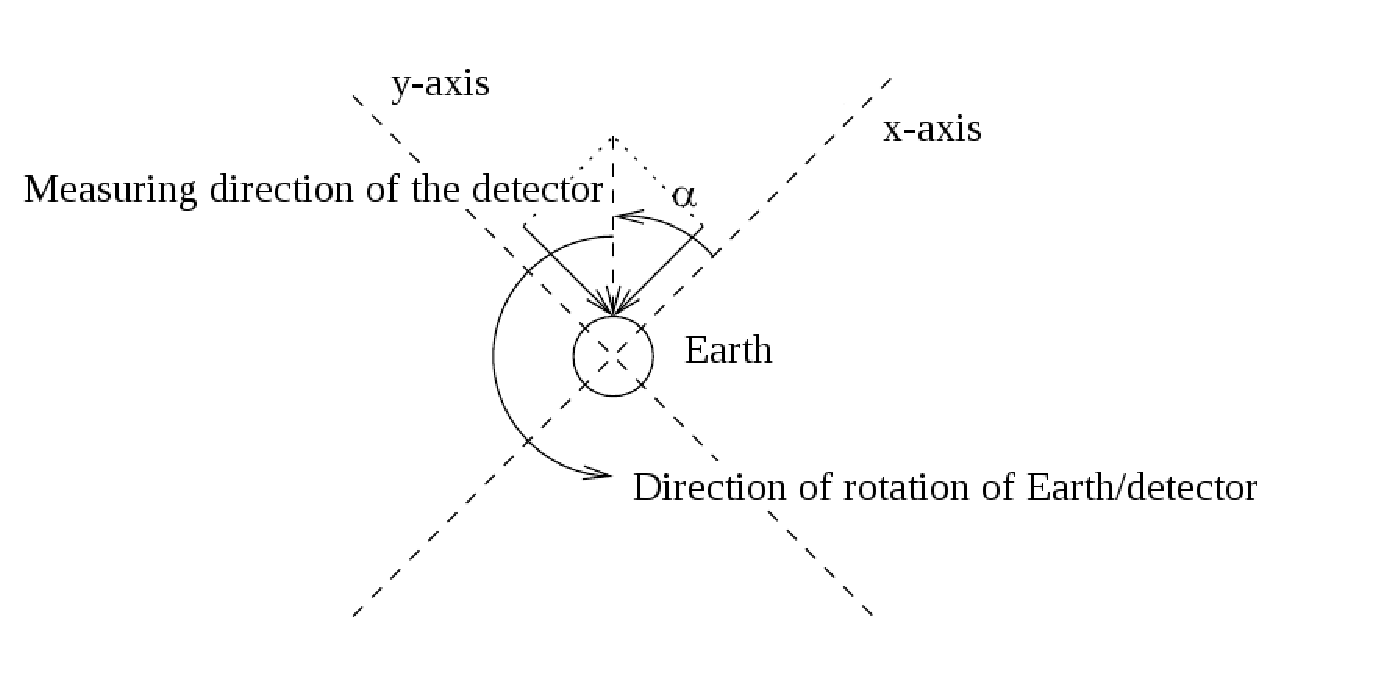
\includegraphics[scale=0.5]{measuring_angle}
\caption{The sky is divided into quadrants and the data is assigned to a quadrant according to the measurement angle $\alpha$.}\label{fig:measuring_angle}
\end{center}\end{figure}

Assigning the data from every hour to the quadrant of figure \ref{fig:measuring_angle} can be done using the following equations:
\begin{align} Data_y &= Data \cdot \sin(\alpha) \\ Data_x &= Data \cdot \cos(\alpha) \end{align}
Or, if we combine these equations with equation \ref{eq:time}:
\begin{align} Data_y &= Data \cdot \sin\left( 2 \pi \frac{t}{T}\right)  \\ Data_x &= Data \cdot \cos(\left( 2 \pi \frac{t}{T}\right) \end{align}
In these equations $Data$ is the total amount of coincidences recorded during a solar hour. $Data_x$ and $Data_y$ represent the data assigned to the quadrants, there is a positive and negative direction making four quadrants.

If the measured cosmic radiation is uniformly distributed over all directions than the sum of $Data_x$ and $Data_y$ of one entire period will be zero. If however there is more radiation coming from a particular direction than at least one of the sums will not be zero. This enables us to point towards a direction of a possible source of cosmic radiation.

This analysis involves a lot of calculations, luckily the spreadsheet programs can do these calculations for us. But first we need to enter the correct formulas and obtain enough data because there is one small caveat: the calculations described above only work with a whole number of periods of data.

\begin{shaded}
\textbf{Exercise \theExercise \stepcounter{Exercise}} : How many solar hours data are needed to obtain a whole number of rotation periods?\end{shaded}

As the last question showed we need a lot of data to make the calculations work. Not only does this involve importing large amount of data (a lot of work) but our detector has to be up and running without problems for the same period of time. To make life a bit easier we will use a shorter period of time. To negate the problems in our analysis caused by the incomplete number of periods used we will assign weighting factors to the data. Data at the start and end of our data set will count less towards the final answer while the middle part will be treated normally. 

The weighting function should be a pure Gauss-curve. However this curve is infinitely long and we already had the problem of insufficient data. Therefore we will use an approximation which can be easily calculated using a spreadsheet program, a raised cosine:
\begin{equation} \mbox{weighting factor} = \frac{1}{2} \left( 1 - \cos\left( 2 \pi \frac{t}{T_m}\right) \right) \end{equation}

\begin{figure}\begin{center}
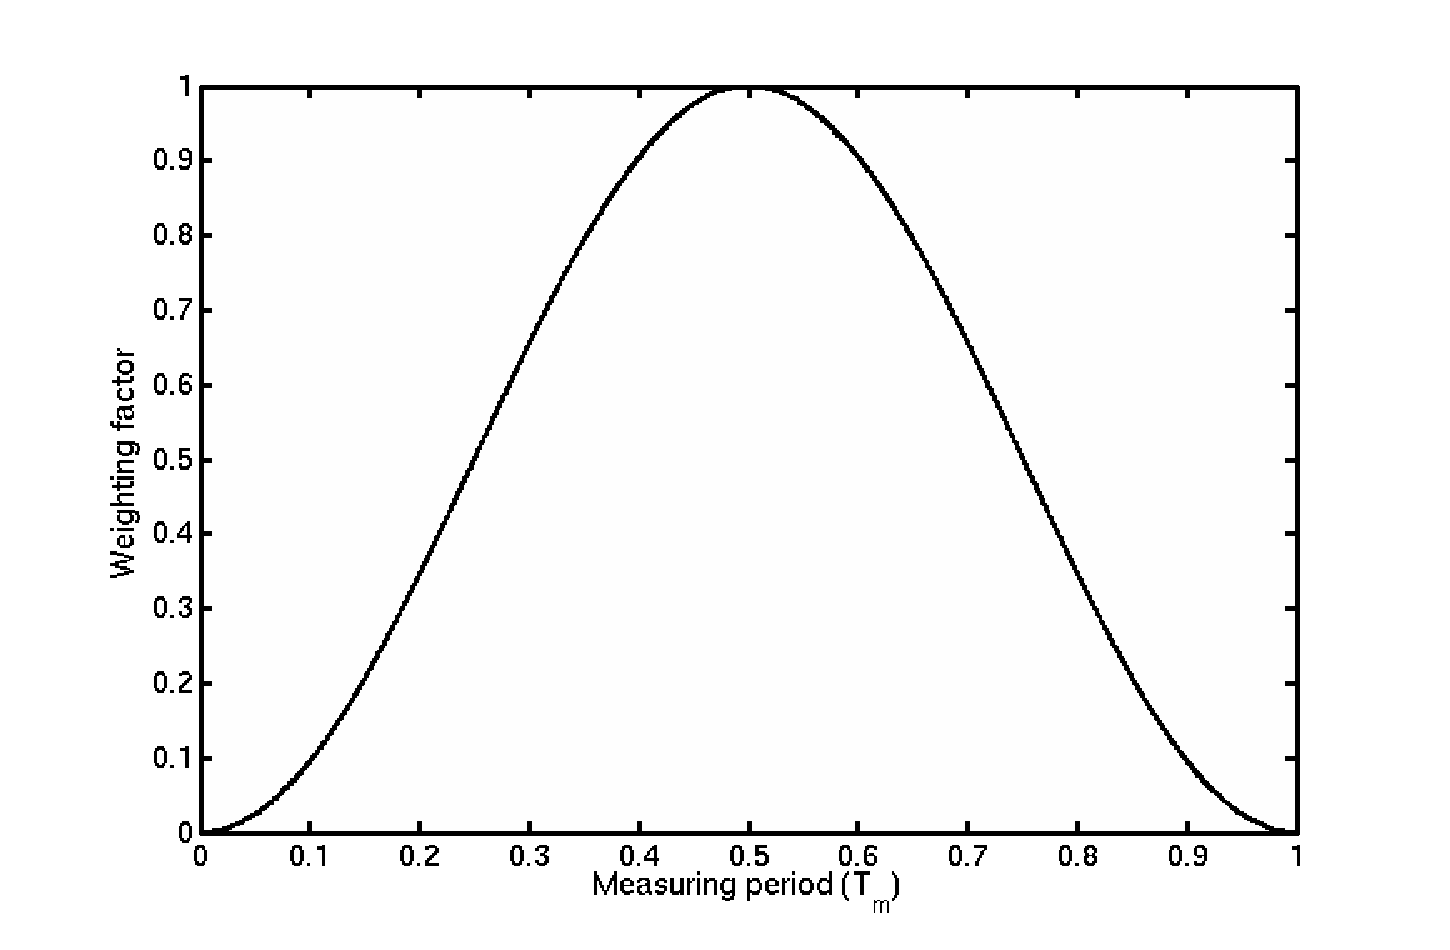
\includegraphics[scale=0.5]{raised_cosine}
\caption{The weighting curve used on the data, a raised cosine.}\label{fig:raised_cosine}
\end{center}\end{figure} 

The entire procedure now becomes:
\begin{enumerate}[1.]
\item Collect the data from a single detector station.
\item Check the validity of the data: Was the detector always on? Are there no strange peaks? Etc.
\item Calculate the duration of a sidereal day.
\item Multiply the data with the raised cosine function to apply weighting.
\item Calculate $Data_x$ and $Data_y$.
\item Determine the sum of $Data_x$ and the sum of $Data_y$.
\end{enumerate}
Are the sums 0? Then there is no direction from where more radiation is detected. Is the sum not 0, then we can take our analysis further. We can use our sums to reconstruct the angle from which the excess of radiation was detected. Lets say we obtained to following sums $\sum Data_x = -525$  and $\sum Data_y = -260$. We can represent this as a line in a coordinate system such as figure \ref{fig:direction}. 

Does this nice line mean their is actually something interesting producing cosmic radiation in the direction of the line? We cannot be sure because charged particles are deflected by magnetic fields. But before we start looking up at the sky, let us first look at the amount of excess radiation. To do this we will compare the amount of radiation coming from the found direction with the total amount of radiation using:
\begin{equation} \mbox{deviation} = \frac{\sqrt{\sum Data_x^2 + \sum Data_y ^2}}{\sum Data} \cdot 100\% \end{equation}

\begin{figure}\begin{center}
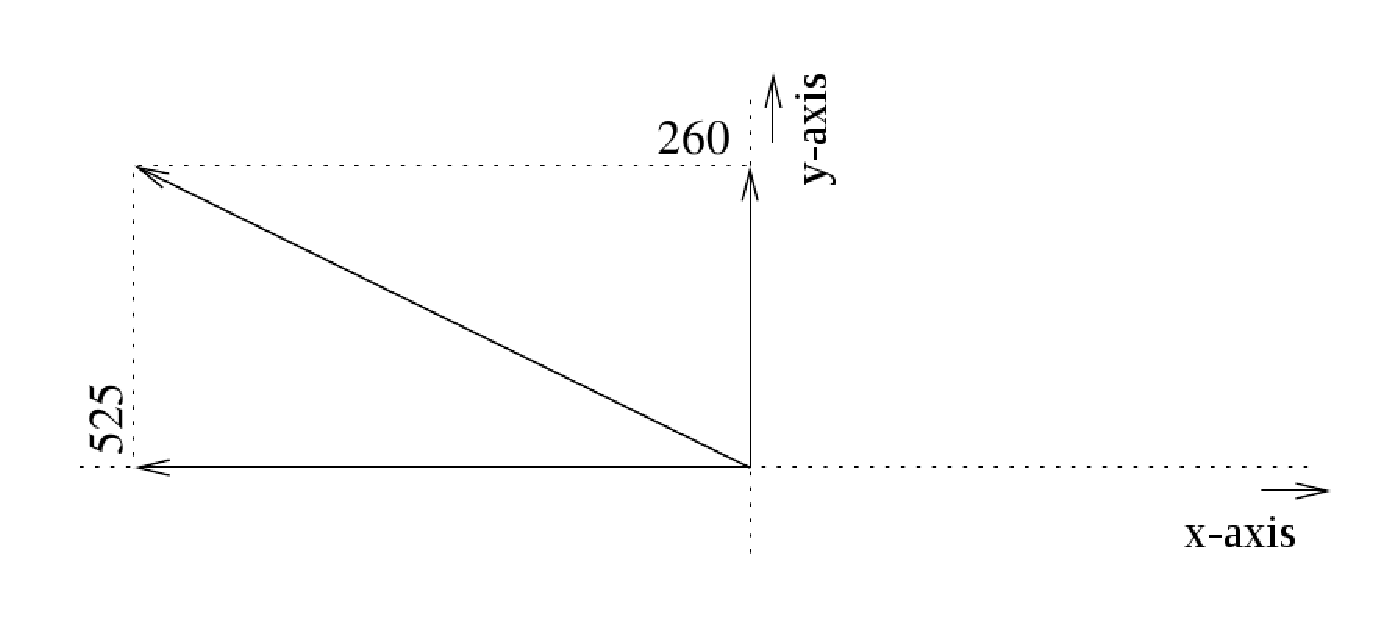
\includegraphics[scale=0.5]{direction}
\caption{The result of the data analysis, the direction of excess radiation is represented as a line.}\label{fig:direction}
\end{center}\end{figure} 

\begin{shaded}
\textbf{Exercise \theExercise \stepcounter{Exercise}} : Use the analysis described above to analyse one week worth of data from your own detector station.\end{shaded}


\end{document}

